\pdfoutput=1
\documentclass[11pt]{article}

% [review] enables line numbers and anonymization for ACL ARR double-blind submission
\usepackage[review]{acl}

\usepackage{times}
\usepackage{latexsym}
\usepackage[T1]{fontenc}
\usepackage[utf8]{inputenc}
\usepackage{microtype}
\usepackage{inconsolata}
\usepackage{graphicx}
\usepackage{booktabs}
\usepackage{multirow}
\usepackage{amsmath}
\usepackage{amssymb}

\title{Does Uncertainty Change Control? A Matched Intervention Study of LLM Action Selection in Biomedical Claim Verification}

\author{Anonymous ACL submission}

\begin{document}
\maketitle

%----------------------------------------------------------------------
\begin{abstract}
\noindent\textbf{Code and data:} \url{https://anonymous.4open.science/r/SOEA-Plus-355B}


Existing evaluations of LLM metacognition typically observe an LLM's answer, uncertainty statement, and action choice together, making it impossible to determine whether the action actually responds to uncertainty. We introduce a \textbf{matched counterfactual intervention} that holds the claim, evidence, and first-order decision fixed while varying only the uncertainty signal available at the control stage. We apply this intervention---the Counterfactual Uncertainty Control Response (CUCR) framework---to three contemporary LLMs (GPT-4.1-mini, Gemini-2.5-Flash, Llama-3.3-70b) on 200 biomedical claim verification cases (PubMedQA). All three models demonstrate significant responsiveness to the uncertainty signal ($\Delta \ge +0.56$), confirming that LLMs can adjust their control behavior when uncertainty is explicitly provided. These findings are situated within a broader evaluation of 1,000 PubMedQA cases across three contemporary LLMs (GPT-4.1-mini, Llama-3.3-70b, Gemini-2.5-Flash), which reveals a consistent Control Collapse Gap (CCG): models commit to incorrect predictions at rates between 70.6\% and 100\%, despite generating uncertainty estimates. Together, these results suggest that LLM control must be tested by intervention, not inferred from co-produced uncertainty.
\end{abstract}

%----------------------------------------------------------------------
\section{Introduction}

The deployment of Large Language Models (LLMs) in safety-critical domains such as biomedicine requires robust metacognitive capabilities. A reliable model must not only generate accurate decisions but also accurately monitor its own uncertainty and, crucially, exert appropriate control---such as abstaining or seeking additional evidence---when uncertainty is high \citep{kadavath2022language, griot2025large}.

However, existing evaluations typically observe an LLM's answer, uncertainty statement, and action choice together within a single prompt or conversation. Such observations cannot determine whether the action actually responds to uncertainty, because all outputs may be co-generated by the same context. A model may report high uncertainty and still not use it to guide its actions; the missing test is counterfactual responsiveness.

In this paper, we test uncertainty-to-control responsiveness by holding the claim, evidence, and first-order decision fixed while counterfactually varying only the uncertainty information available at the control stage. This design turns uncertainty use from an inferred correlation into a directly testable behavioral outcome.

Our contributions are threefold:
\begin{enumerate}
    \item \textbf{A Scaled Metacognitive Evaluation:} We evaluate 1,000 biomedical claim-evidence pairs from PubMedQA across three contemporary LLMs under both single-prompt (Protocol A) and multi-turn (Protocol B) elicitation, revealing a consistent Control Collapse Gap (CCG) across all models.
    \item \textbf{Supporting SOEA-Plus Analysis:} We report PDEMC (a composite score integrating Decision Accuracy, Monitoring Fidelity, and Control Rationality) and weight sensitivity analysis as supporting evidence for the broader evaluation. The main contribution of this work is the CUCR intervention; PDEMC serves as a structured lens for interpreting the observational results.
    \item \textbf{The CUCR Intervention Framework:} A matched counterfactual intervention that holds claim, evidence, and decision fixed while varying only the imposed uncertainty signal. Applied to three contemporary LLMs across $N=200$ PubMedQA cases, CUCR reveals strong behavioral responsiveness in all evaluated models ($\Delta \ge +0.56$), providing direct intervention-based evidence that uncertainty-to-control responsiveness can be measured and is significant.
\end{enumerate}

%----------------------------------------------------------------------
\section{Related Work}

\subsection{Calibration and Uncertainty Estimation}
The problem of model calibration has received substantial attention. \citet{guo2017calibration} demonstrated that modern neural networks are systematically overconfident, proposing temperature scaling as a post-hoc remedy. \citet{jiang2021calibration} showed that verbalized confidence in language models does not reliably correlate with accuracy. \citet{tian2023just} further demonstrated that instruction-tuned models exhibit complex calibration patterns that vary by task type, while \citet{xiong2024llms} evaluated black-box confidence elicitation, finding that models tend toward overconfidence but improve with scale. These works evaluate whether uncertainty estimates are calibrated, but they do not determine whether the model's downstream action changes when uncertainty alone is manipulated.

\subsection{Selective Prediction and Abstention}
Selective prediction \citep{geifman2017selective} allows models to abstain when uncertain, trading coverage for accuracy. \citet{kamath2020selective} applied this to question answering under domain shift, demonstrating that softmax probabilities alone are insufficient. \citet{varshney2022investigating} evaluated selective prediction across numerous datasets, finding that methods do not consistently outperform MaxProb. Recently, \citet{presacan2026when} reviewed LLM abstention in healthcare, proposing a decision-theoretic framework for safety-driven abstention. Selective prediction studies answer whether a model should answer or abstain; our setting generalizes control to multiple actions and tests uncertainty responsiveness through a matched intervention.

\subsection{Metacognition and the Knowing-Doing Gap}
\citet{kadavath2022language} introduced self-evaluation as a metacognitive probe, finding that large models can assess their own correctness. However, \citet{griot2025large} demonstrated that current LLMs exhibit a critical disconnect between perceived and actual capabilities in medical reasoning. \citet{wang2026mirror} identified a ``knowing-doing gap'' in LLMs, showing that providing models their own uncertainty does not reliably improve their control decisions. \citet{zhang2026calibration} argued theoretically that calibration is not control, calling for intervention-based evaluations. Closest to our work, these two studies argue that self-knowledge and calibration do not guarantee appropriate action. CUCR differs by introducing a matched intervention in biomedical claim verification, holding the claim, evidence, and first-order decision fixed while varying only the uncertainty signal.

\subsection{Biomedical Claim Verification}
We evaluate our framework on PubMedQA \citep{jin2019pubmedqa}, a dataset of expert-labeled biomedical research questions. Similar tasks include SciFact \citep{wadden2020fact}, which verifies scientific claims against research abstracts. Biomedical claim verification provides a high-stakes testbed where incorrect commitment under uncertainty is especially consequential. To our knowledge, no prior work has directly tested uncertainty-to-control responsiveness in biomedical claim verification using a matched intervention that holds claim, evidence, and first-order decision fixed while varying only the uncertainty signal.

%----------------------------------------------------------------------
\section{Methodology}

\subsection{The SOEA-Plus Three-Stage Protocol}
SOEA-Plus evaluates LLMs through three sequential stages applied to each biomedical claim-evidence pair:

\textbf{Stage 1 --- Decision.} The model classifies the claim as \textsc{Supported}, \textsc{Refuted}, or \textsc{Inconclusive} based on the provided evidence.

\textbf{Stage 2 --- Monitoring.} The model provides an error probability $p \in [0, 1]$, where $p = 0$ indicates certainty of correctness and $p = 1$ indicates certainty of error.

\textbf{Stage 3 --- Control.} Based on its decision and error probability, the model selects one of four explicitly defined actions:
\begin{itemize}
    \item \textbf{\textsc{Commit}:} Proceed with the current decision; appropriate when uncertainty is low and the decision is reliable.
    \item \textbf{\textsc{Revise}:} Change the current decision; appropriate when evidence appears to contradict the decision.
    \item \textbf{\textsc{Abstain}:} Decline to provide a decision; appropriate when uncertainty is too high to commit safely.
    \item \textbf{\textsc{Seek\_Evidence}:} Request additional evidence; appropriate when current evidence is insufficient or ambiguous.
\end{itemize}

We evaluate this under two protocols: \textbf{Protocol A} (single-prompt, all stages elicited jointly, N=1,000) and \textbf{Protocol B} (multi-turn, stages elicited sequentially to prevent self-conditioning bias, N=200).

\subsection{The PDEMC Metric}
The PDEMC score integrates all three stages:
\begin{equation}
\text{PDEMC} = 0.30 \times \text{Acc} + 0.30 \times \text{MF} + 0.40 \times \text{CR}
\end{equation}
where Acc is Stage 1 accuracy, MF (Monitoring Fidelity) is $1 - \text{MAE}(p_i, e_i)$ (with $e_i = 1$ if the Stage 1 decision is incorrect, and $0$ otherwise), and CR (Control Rationality) is defined as:
\begin{equation}
\text{CR} = 
\begin{cases} 
1 & \text{if } (\hat{y}_i = y_i \wedge a_i = \textsc{Commit}) \\
  & \vee (\hat{y}_i \neq y_i \wedge a_i \in \{\textsc{Revise}, \textsc{Abstain}, \textsc{Seek}\}) \\
0 & \text{otherwise}
\end{cases}
\end{equation}
Control receives the highest weight (40\%) as the safety-critical output, while Accuracy and Monitoring Fidelity are weighted equally (30\% each) to balance first-order correctness with self-awareness. PDEMC collapses these three dimensions into a single ranking-stable score, enabling robust cross-study comparison and sensitivity analysis. Sensitivity analysis over four alternative weight configurations confirms that model rankings are stable across all configurations (see Section~\ref{sec:sensitivity}).

\subsection{The Control Collapse Gap}
The Control Collapse Gap (CCG) quantifies the rate at which models commit to incorrect predictions:
\begin{equation}
\text{CCG} = \frac{|\{i : \hat{y}_i \neq y_i \wedge a_i = \textsc{Commit}\}|}{|\{i : \hat{y}_i \neq y_i \}|}
\end{equation}
A high CCG indicates that even when a model is wrong, it overwhelmingly chooses to commit rather than abstain or revise.

\subsection{The CUCR Intervention}
To provide intervention-based behavioral evidence that the CCG reflects a failure of control rather than merely poor calibration, we introduce the Counterfactual Uncertainty Control Response (CUCR) framework. For each evaluated sample, we hold the claim, evidence, and first-order decision fixed, and inject an imposed uncertainty level $U_{\text{imposed}} \in \{0.10, 0.30, 0.50, 0.70, 0.90\}$ into the prompt, asking the model to select a control action given this specific value. These five levels were chosen to provide evenly spaced intervals covering the full probability range. We also include a \textit{masked} condition in which no uncertainty value is provided, serving as a baseline. If the model behaviorally uses the supplied uncertainty signal, its Safe Action Rate should rise monotonically with $U_{\text{imposed}}$.

We evaluate the CUCR protocol on a subset of 200 cases from PubMedQA to ensure robust statistical power. We measure responsiveness via $\Delta = (U=0.9) - (U=0.1)$, capturing the maximum behavioral shift across the uncertainty spectrum.

\subsection{Dataset and Models}
We evaluate on 1,000 claim-evidence pairs sampled from PubMedQA \citep{jin2019pubmedqa} (seed=42, \texttt{pqa\_labeled} split), with labels mapped from \{yes, no, maybe\} to \{\textsc{Supported}, \textsc{Refuted}, \textsc{Inconclusive}\}. The same 1,000 cases are used across all models and conditions. Main SOEA-Plus evaluation uses GPT-4.1-mini, Llama-3.3-70b, and Gemini-2.5-Flash. These three models were selected to represent distinct providers (OpenAI, Meta/Groq, Google) and span a range of parameter scales and training paradigms; cross-model comparisons in Table~\ref{tab:main_results} should be interpreted as provider-level baselines rather than controlled scale comparisons. The CUCR intervention uses GPT-4.1-mini, Gemini-2.5-Flash, and Llama-3.3-70b.

%----------------------------------------------------------------------
\section{Main Results}

\subsection{Protocol A: Control Collapse Across Models (N=1,000)}

Table~\ref{tab:main_results} presents the main results. GPT-4.1-mini achieves the highest accuracy (46.2\%) but exhibits a CCG of 70.6\%. Llama-3.3-70b shows a CCG of 91.2\%, while Gemini-2.5-Flash commits to every incorrect prediction (CCG = 100\%), completely ignoring its own mean error probability of 0.500. Figure~\ref{fig:pdemc} visualizes the PDEMC component breakdown, highlighting that low Control Rationality (CR) is the primary driver of poor overall performance across all models.

\begin{figure}[h]
    \centering
    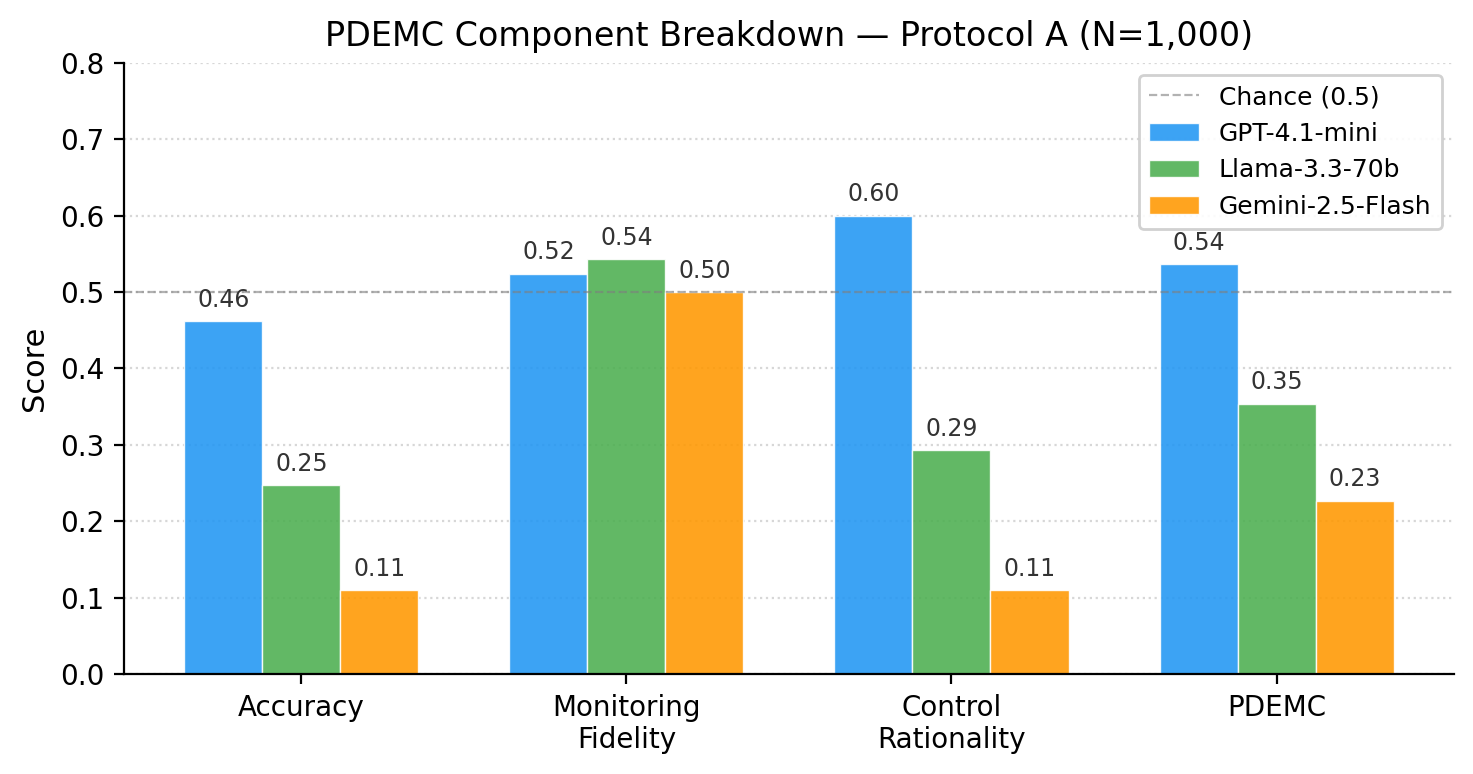
\includegraphics[width=\linewidth]{pdemc_components.png}
    \caption{PDEMC component breakdown (Protocol A). While Accuracy and Monitoring Fidelity vary, Control Rationality remains the weakest component for all models except GPT-4.1-mini.}
    \label{fig:pdemc}
\end{figure}

\begin{table}[h]
\centering
\small
\begin{tabular}{lcccc}
\toprule
\textbf{Model} & \textbf{Acc} & \textbf{Safe} & \textbf{CCG} & \textbf{PDEMC} \\
\midrule
GPT-4.1-mini & 0.462 & 0.178 & 70.6\% & 0.536 \\
Llama-3.3-70b & 0.247 & 0.086 & 91.2\% & 0.354 \\
Gemini-2.5-Flash & 0.110 & 0.000 & 100.0\% & 0.227 \\
\bottomrule
\end{tabular}
\caption{Main results, Protocol A (N=1,000, seed=42). Safe = safe action rate (ABSTAIN + REVISE + SEEK\_EVIDENCE). 95\% CIs: GPT Acc [0.432--0.491], Llama Acc [0.222--0.276], Gemini Acc [0.092--0.131].}
\label{tab:main_results}
\end{table}

\subsection{Protocol Comparison (N=200)}

Table~\ref{tab:protocol} compares single-prompt (Protocol A, N=1,000) vs.\ multi-turn (Protocol B, N=200) elicitation. Because Protocol B requires three sequential API calls per case, it was applied to the first 200 cases of the dataset; Protocol A numbers in this table reflect the full N=1,000 evaluation. As visualized in Figure~\ref{fig:protocol}, Llama-3.3-70b shows a substantial improvement under Protocol B: accuracy rises from 0.247 to 0.425, and the safe action rate increases from 8.6\% to 39.5\% (+31 percentage points). This suggests that staged elicitation, which forces the model to articulate its uncertainty before selecting an action, meaningfully improves control responsiveness. GPT-4.1-mini and Gemini-2.5-Flash show minimal protocol sensitivity.

\begin{figure}[h]
    \centering
    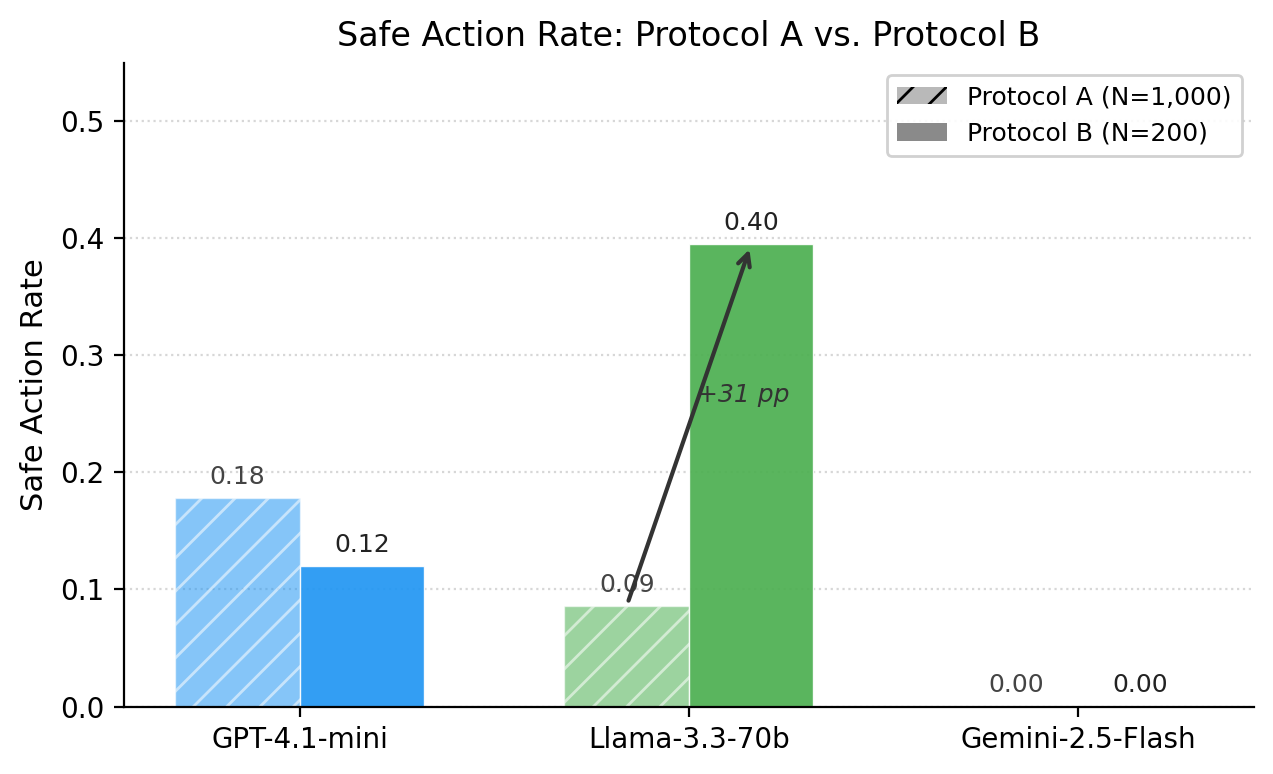
\includegraphics[width=0.9\linewidth]{protocol_comparison.png}
    \caption{Safe Action Rate comparison between Protocol A (single-prompt) and Protocol B (multi-turn). Llama-3.3-70b exhibits a dramatic +31 percentage point improvement under staged elicitation.}
    \label{fig:protocol}
\end{figure}

\begin{table}[h]
\centering
\small
\begin{tabular}{llccc}
\toprule
\textbf{Model} & \textbf{Protocol} & \textbf{Acc} & \textbf{Safe} & \textbf{Commit} \\
\midrule
\multirow{2}{*}{GPT-4.1-mini} & A (N=1,000) & 0.462 & 0.178 & 0.822 \\
 & B (N=200) & 0.460 & 0.120 & 0.880 \\
\midrule
\multirow{2}{*}{Llama-3.3-70b} & A (N=1,000) & 0.247 & 0.086 & 0.914 \\
 & B (N=200) & 0.425 & 0.395 & 0.605 \\
\midrule
\multirow{2}{*}{Gemini-2.5-Flash} & A (N=1,000) & 0.110 & 0.000 & 1.000 \\
 & B (N=200) & 0.075 & 0.000 & 1.000 \\
\bottomrule
\end{tabular}
\caption{Protocol A (N=1,000) vs.\ Protocol B (N=200). Protocol B was applied to a 200-case subset due to its multi-turn cost. Acc = accuracy, Safe = safe action rate (ABSTAIN + REVISE + SEEK), Commit = overall commit rate (= 1 $-$ Safe). Note: Commit rate differs from CCG (Table~\ref{tab:main_results}), which conditions on incorrect predictions only.}
\label{tab:protocol}
\end{table}

\subsection{Sensitivity Analysis}
\label{sec:sensitivity}

Table~\ref{tab:sensitivity} reports PDEMC scores under four alternative weight configurations. Model rankings remain identical across all configurations, confirming that the PDEMC metric is robust to reasonable weight perturbations.

\begin{table}[h]
\centering
\small
\begin{tabular}{lccc}
\toprule
\textbf{Weights (Acc/MF/CR)} & \textbf{GPT} & \textbf{Llama} & \textbf{Gemini} \\
\midrule
30/30/40 (original) & 0.536 & 0.354 & 0.227 \\
33/33/34 (equal) & 0.529 & 0.360 & 0.239 \\
25/25/50 (control-heavy) & 0.547 & 0.344 & 0.208 \\
50/25/25 (accuracy-heavy) & 0.512 & 0.333 & 0.208 \\
\bottomrule
\end{tabular}
\caption{PDEMC sensitivity analysis. Rankings are stable across all configurations.}
\label{tab:sensitivity}
\end{table}

\subsection{Error Analysis (N=3,600)}

A comprehensive audit of 3,600 evaluated rows (3 models $\times$ 1,000 Protocol A + 3 models $\times$ 200 Protocol B) categorized five failure types (Table~\ref{tab:error}). The dominant failure mode is ``Uncertainty ignored'' (48.6\%)---defined as committing to an incorrect prediction despite reporting an error probability $p \geq 0.30$---confirming that models frequently fail to translate their uncertainty estimates into appropriate control actions. ``High-confidence wrong commit'' (15.3\%)---where the model makes an incorrect prediction, reports low uncertainty ($p < 0.30$), and commits---represents the most critical safety risk in high-stakes settings.

\begin{table}[h]
\centering
\small
\begin{tabular}{lcc}
\toprule
\textbf{Failure Type} & \textbf{Count} & \textbf{\%} \\
\midrule
Uncertainty ignored & 1749 & 48.6\% \\
Safe correct commit & 935 & 26.0\% \\
High-confidence wrong commit & 549 & 15.3\% \\
Safe response to wrong decision & 291 & 8.1\% \\
Over-cautious safe action & 76 & 2.1\% \\
\bottomrule
\end{tabular}
\caption{Error analysis of 3,600 evaluated rows.}
\label{tab:error}
\end{table}

%----------------------------------------------------------------------
\section{The CUCR Pilot Intervention}

\subsection{Results: Natural, Masked, and Intervention Conditions}

Table~\ref{tab:cucr_full} presents the complete CUCR results across all conditions. The \textit{natural} condition shows the baseline safe action rate from joint elicitation; the \textit{masked} condition shows the rate when no uncertainty value is provided; the intervention conditions show the rate at each imposed uncertainty level.

\begin{table*}[t]
\centering
\small
\begin{tabular}{l|c|ccccc|c}
\toprule
\textbf{Model} & \textbf{Masked} & \textbf{U=0.1} & \textbf{U=0.3} & \textbf{U=0.5} & \textbf{U=0.7} & \textbf{U=0.9} & \textbf{$\Delta$} \\
\midrule
GPT-4.1-mini & .640 & .330 & .745 & .775 & .910 & .890 & +.560 \\
Gemini-2.5-Flash & .415 & .280 & .455 & .750 & .875 & .910 & +.630 \\
Llama-3.3-70b & .395 & .375 & 1.000 & 1.000 & 1.000 & 1.000 & +.625 \\
\bottomrule
\end{tabular}
\caption{CUCR Response Table ($N=200$, deduplicated). Safe Action Rate across uncertainty conditions. $\Delta$ = Safe Rate at $U=0.9$ $-$ Safe Rate at $U=0.1$. 95\% CIs: GPT $\Delta$ [0.491, 0.629]; Gemini $\Delta$ [0.563, 0.697]; Llama-70b $\Delta$ [0.558, 0.692]. Note: Llama-3.1-8b expansion did not complete ($N=3$ valid cases) and is excluded from analysis.}
\label{tab:cucr_full}
\end{table*}

\begin{figure}[h]
    \centering
    
\includegraphics[width=\linewidth]{cucr_response_curves.png}
    \caption{CUCR response curves ($N=200$). All three models demonstrate significant responsiveness to the uncertainty signal, but with distinct behavioral curves.}
    \label{fig:cucr}
\end{figure}

\subsection{Model Divergence in Control Responsiveness}

All three models demonstrate significant responsiveness to the uncertainty signal, confirming the core hypothesis that LLMs can adjust their control behavior when uncertainty is explicitly provided.

Llama-3.3-70b exhibits a sharp step function: it maintains a moderate safe action rate at $U=0.1$ (0.375), but immediately reaches 1.000 at $U \ge 0.3$. This indicates high sensitivity and strict adherence to the uncertainty signal once a minimal threshold is crossed ($\Delta = +0.625$, 95\% CI [0.558, 0.692]).

GPT-4.1-mini and Gemini-2.5-Flash show more gradual, monotonic response curves. GPT-4.1-mini scales its safe action rate from 0.330 at $U=0.1$ to 0.890 at $U=0.9$ ($\Delta = +0.560$, 95\% CI [0.491, 0.629]). Gemini-2.5-Flash scales from 0.280 to 0.910 ($\Delta = +0.630$, 95\% CI [0.563, 0.697]).

The Llama-3.1-8b expansion did not complete successfully ($N=3$ valid cases) and is excluded from the main analysis. Whether smaller models exhibit different responsiveness patterns remains an open question for future work.

%----------------------------------------------------------------------
\section{Discussion}

Our results indicate that explicit uncertainty and behavioral control are separable. The CUCR intervention provides direct behavioral intervention evidence that models can align their actions with an imposed uncertainty signal when it is explicitly provided, even if they fail to do so when generating the uncertainty themselves (as seen in the CCG results).

We acknowledge that CUCR measures behavioral responsiveness to an explicit numerical signal; whether this reflects genuine metacognitive use of uncertainty or sophisticated instruction-following is a question for future mechanistic work. However, the \textit{masked} condition provides partial evidence against pure instruction-following: without a numerical signal, models revert to a stable default behavior (masked safe rates: GPT 0.640, Gemini 0.415, Llama-70b 0.395) rather than random selection, indicating that the injected number shifts an existing behavioral baseline. Crucially, for deployed systems where uncertainty is communicated numerically (e.g., via calibration pipelines), behavioral responsiveness to the signal is the operationally relevant test.

The stark contrast in Llama-3.3-70b's behavior between Protocol A and Protocol B further suggests that control responsiveness is highly protocol-moderated. This underscores the need for intervention-based evaluations rather than relying solely on co-produced uncertainty statements. Gemini-2.5-Flash's degenerate behavior (CCG = 100\% in natural settings) further highlights that some models appear to completely decouple their stated uncertainty from their action policy.

%----------------------------------------------------------------------
\section{Limitations}

This study evaluates behavioral responsiveness, not mechanistic internal cognition. The primary testbed is biomedical claim verification (PubMedQA), and results may vary in other domains. The evaluation relies on API-based models, which are subject to versioning changes. The CUCR intervention uses N=200 samples per model; future work should scale this to the full 1,000-sample set and extend the intervention to additional model families. The Llama-3.1-8b expansion did not complete successfully and is excluded from the main CUCR analysis; future work should repeat the intervention across additional model sizes to assess scale effects. The intervention manipulates only the uncertainty signal while leaving the semantic content of the claim and evidence unchanged; future work should explore whether manipulating other contextual signals produces similar effects. Human-level PDEMC baselines are not directly measured and are left for future annotation studies.

%----------------------------------------------------------------------
\section*{Data Availability}
All code, data, and results are available at \url{https://anonymous.4open.science/r/SOEA-Plus-355B}.

\section{Conclusion}

LLM control must be tested by intervention, not inferred from co-produced uncertainty. Our matched counterfactual intervention reveals a significant gap between uncertainty awareness and control responsiveness, with a scale-dependent divergence: the evaluated models show significant behavioral responsiveness when uncertainty is explicitly provided, yet fail to use their own uncertainty estimates in natural settings. The prevalence of ``Uncertainty ignored'' failures (48.6\%) across the broader 1,000-sample evaluation demonstrates that calibration alone is insufficient as an evaluation criterion for high-stakes deployment.

\section*{Acknowledgments}
Anonymized for review.

\bibliography{custom}

\end{document}
